\documentclass[11pt,reqno]{amsart}
\usepackage{epsfig}
\usepackage{graphicx}
\usepackage{booktabs}
\usepackage{amsfonts}
\usepackage{amsmath}
\usepackage{amssymb}
%\usepackage{mathrsfs}
\usepackage{hyperref}
\setcounter{MaxMatrixCols}{10}
\hfuzz=12pt
\hbadness=5000
\vbadness=5000
\frenchspacing
\vfuzz=2pt
\input{epsf}
%\input{tcilatex}

\begin{document}

\title[Bootstrapping the Illiquidity]{Bootstrapping the Illiquidity \\ \footnotesize{\emph{Post Credit Crunch Multiple Yield Curves Construction \\
For Market Coherent Smooth Forward Rates Estimation}}}

\author{Ferdinando M. Ametrano}
\address{Financial Engineering, Banca IMI, Piazzetta G. Dell'Amore 3, 20121
Milan Italy, ferdinando.ametrano(AT)bancaimi.com}

\author{Marco Bianchetti}
\address{Risk Management, Banca IntesaSanpaolo, Piazza G. Ferrari 10, 20121
Milan Italy, marco.bianchetti(AT)intesasanpaolo.com}

\thanks{JEL Classifications: E45, G13. \\
The authors acknowledge fruitful discussions with S. De Nuccio, R. Giura, C. Maffi, F. Mercurio, N. Moreni and the QuantLib community. The opinions expressed here are solely of the authors and do not represent in any way those of theirs employers.}

\date{Draft Feb. 14th, 2008}

\keywords{liquidity, crisis, interest rates, yield curve, forward curve, discount curve, bootstrapping, pricing, hedging, interest rate derivatives, FRAs, Futures, Swaps, Basis Swaps, QuantLib.}

\begin{abstract}
The large basis spreads observed on the interest rate market since the liquidity crisis of summer 2007 imply that different yield curves are required for market coherent estimation of forward rates with different tenors (e.g. Euribor 3 months, Euribor 6 months, etc.).
\\ In this paper we review in detail the methodology for bootstrapping interest rate yield curves from plain vanilla derivatives quoted on the market.
In particular we describe how to extract multiple yield curve term structures, each homogeneous in the underlying rate tenor, from non-homogeneous instruments such as Deposits, Forward Rate Agreements, Futures, Swaps, and Basis Swaps. The approach includes turn-of-year effects and is robust to deliver smooth yield curves and to ensure non-negative rates also in highly stressed market situations, characterized by crazy roller coaster shapes of the market quotations.
\\ The concrete EUR market case is analyzed in detail, using the open source QuantLib implementation of the proposed algorithms.
\end{abstract}

\maketitle
\tableofcontents

\section{Introduction}
\label{sec:Intro}
Pricing complex interest rate derivatives requires modeling the future dynamics of the yield curve term structure. Most of the literature assumes the existence of the \emph{current} yield curve as given, and its construction is often neglected, or even obscured, as it is considered more an art than a science. Actually any yield curve term structure modeling approach will fail to produce good/reasonable prices if the current term structure is not correct.
\par
Financial institutions, software houses and practitioners have developed various methodologies in order to extract the yield curve term structure from quoted prices of a finite number of liquid market instruments.
\textquotedblleft Best-fit\textquotedblright\ algorithms assume a smooth functional form for the term structure and calibrate its parameters such that to minimize the repricing error of the chosen set of calibration instruments. For instance, the European Central Bank publishes yield curves on the basis of the Soderlind and Svensson model \cite{SodSwe1997}, which is an extension of the Nelson-Siegel model (see e.g. refs. \cite{NelSie1987}, \cite{Diament}, \cite{ChrDie07} and \cite{Cor08}). Such approach is popular due to the smoothness of the curve, calibration easiness, intuitive financial interpretation of functional form parameters (level, slope, curvature) and correspondence with principal component analysis. On the other side, the fit quality is typically not good enough for trading purposes in liquid markets.
\par
In practice \textquotedblleft exact-fit\textquotedblright\ algorithms are often preferred: they fix the yield curve on a time grid of $N$ points (pillars) in order to \emph{exactly} reprice $N$ pre-selected market instruments. The implementation of such algorithms is often incremental, extending the yield curve step-by-step with the increasing maturity of the ordered instruments, in a so called \textquotedblleft bootstrap\textquotedblright approach. Intermediate yield curve values are obtained by interpolation on the bootstrapping grid. Here different interpolation algorithms are available but little attention has been devoted in the literature to the fact that interpolation is often already used during bootstrapping, not just after that, and that the interaction between bootstrapping and interpolation can be subtle if not nasty (see e.g. \cite{HagWes06}, \cite{HagWes08}).
\par
Whilst naive algorithms may fail to deal with market subtleties such as date conventions, the intra-day fixing of the first floating payment of a Swap, the turn-of-year effect, the Futures convexity adjustment, etc., even very sophisticated algorithms used in a naive way may fail to estimate correct forward Euribor rates in difficult market conditions. Namely using just one single curve is not enough to account for forward Euribor rates of different tenor, such as 1, 3, 6, 12 months, because of the large Basis Swap spreads observed since the summer of 2007 in occasion of the so-called {\it subprime credit crunch crisis.}
\par
The plan of the paper is as follows:
in section \ref{sec:Pricing} we start by reviewing the traditional (old style) single curve market practice for pricing and hedging interest rate derivatives and the recent market evolution, triggered by the credit crunch crisis, towards a double-curve approach.
In section \ref{sec:Math} we fix the notation and nomenclature.
In section \ref{sec:SingleBootstrapping} we summarize the traditional pre-credit crunch yield curve construction methodology.
In section \ref{sec:MultiBootstrapping}, that constitutes the central contribution of this work, we describe in great detail the new post-credit crunch multi-curve approach; in particular in its six subsections we discuss the general features of the bootstrapping procedure, we review the (EUR) market instruments available for the bootstrap, and we deal with issues crucial for smooth curve bootstrapping:
the fundamental role of interpolation (\ref{sec:Interp}),
the treatment of priorities and of the overlapping points at different market instruments sections (\ref{sec:DepoFuturesOverlap}),
the incorporation of the turn-of-year effect (\ref{sec:TOY}),
the construction of the underspecified first period coherently with interpolated market FRAs (\ref{sec:Synt}).
Then, in section \ref{sec:ImplementResults} we describe the numerical results delivered by the proposed framework, along with a quick overview of the corresponding open-source QuantLib implementation and of its Excel interface, able to bootstrap multiple yield curves in real-time for real-life needs.
Finally, in section \ref{sec:Pricing2curves} we take a look of the consequences of using different curves for calculating forward rates and discount factors on no arbitrage conditions and on pricing expression for interest rate derivatives.
The conclusions are collected in section \ref{sec:Conclusions}.

\section{Pre and Post Credit Crunch Pricing \& Hedging Interest Rate Derivatives}
\label{sec:Pricing}
One of the many consequences of the credit and liquidity crisis started in the second half of 2007 has been a strong increase of the basis spreads quoted on the market between single-currency interest rate instruments, Swaps in particular, characterized by different underlying rate tenors (e.g. Euribor3M\footnote{Euro Interbank Offered Rate, the rate at which euro interbank term Deposits within the euro zone are offered by one prime bank to another prime bank (see e.g. www.euribor.org).}, Euribor6M, etc.), reflecting the increased liquidity risk and the corresponding preference of financial institutions for receiving payments with higher frequency (quarterly instead of semi-annualy, for instance).
\par
There are also other indicators of regime changes in the interest rate markets, such as the divergence between Deposit (Euribor based) and OIS (Overnight Indexed Swaps, Eonia\footnote{Euro OverNight Index Average, the rate computed as a weighted average of all overnight rates corresponding to unsecured lending transactions in the euro-zone interbank market (see e.g. \url{http://www.euribor.org}).} based) rates with the same maturity, or between FRA (Forward Rate Agreement) contacts and the corresponding forward rates implied by consecutive Deposits.
\par
The asymmetries cited above have also induced a sort of "segmentation" of the interest rate market into sub-areas, mainly corresponding to instruments with 1M, 3M, 6M, 12M underlying rate tenors, characterized, in principle, by different internal dynamics, liquidity and credit risk premia, reflecting the different views and interests of the market players. We stress that such new market situation is nothing else that a new equilibrium configuration determined by the pressure of the increased illiquidity force, that magnifies well known effects historically very small and traditionally neglected before the crisis (see also the discussion in refs. \cite{Mor08}, \cite{Mer09}).
\par
The evolution of the financial markets briefly described above has triggered a general reflection about the methodology used to price and hedge interest rate derivatives, namely those financial instruments whose price depends on the present value of future interest rate-linked cashflows.

\subsection{\label{sec:SingleCurve}The Traditional Single Curve Approach}
\par
The pre-crisis standard market practice (which does not automatically mean good practice) can be summarized in the following procedure (see e.g. refs. \cite{Ron00}, \cite{HagWes06}, \cite{And07} \cite{HagWes08}):
\begin{enumerate}
\item select \emph{one} finite set of the most convenient (e.g. liquid) vanilla interest rate instruments traded in real time on the market with increasing maturities; for instance, a very common choice in the EUR market is a combination of short-term EUR Deposit, medium-term Futures on Euribor3M and medium-long-term Swaps on Euribor6M;

\item build \emph{one} yield curve using the selected instruments plus a set of bootstrapping rules (e.g. pillars, priorities, interpolation, etc.);

\item compute \emph{on the same curve} forward rates, cashflows\footnote{within the present context of interest rate derivatives we focus in particular on forward rate dependent cashflows.}, discount factors and work out the prices by summing up the discounted cashflows;

\item compute the delta sensitivity and hedge the resulting delta risk using the suggested amounts (hedge ratios) of the \emph{same} set of vanillas.
\end{enumerate}
For instance, a 5.5Y maturity EUR floating Swap leg on Euribor1M (not directly quoted on the market) is commonly priced using discount factors and forward rates calculated on the same Depo-Futures-Swap curve cited above. The corresponding delta sensitivity is calculated by shocking one by one the curve pillars and the resulting delta risk is hedged using the suggested amounts (hedge ratios)\ of 5Y and 6Y Euribor6M Swaps\footnote{we refer here to the case of local yield curve bootstrapping methods, for which there are no sensitivity delocalization effect (see refs. \cite{HagWes06}, \cite{And07} \cite{HagWes08}).}.
\par
We stress that this is a \emph{single-currency-single-curve approach}, in that a \emph{unique} curve is built and used to price and hedge any interest rate derivative on a given currency. Thinking in terms of more fundamental variables, e.g. the short rate, this is equivalent to assume that there exist a unique fundamental underlying short rate process able to model and explain the whole term structure of interest rates of any tenor.
\par
It is also a \emph{relative pricing} approach, because both the price and the hedge of a derivative are calculated relatively to a set of vanillas quoted on the market. We notice also that the procedure is not strictly guaranteed to be arbitrage-free, because discount factors and forward rates obtained through interpolation are, in general, not necessarily consistent with the no arbitrage condition; in practice bid-ask spreads and transaction costs virtually hide any arbitrage possibility.
\par
Finally, we stress that the first key point in the procedure above is much more a matter of art than of science, because there is not an unique financially sound choice of bootstrapping instruments and, in principle, none is better than the others.
\par
The pricing \& hedging methodology described above can be extended, in principle, to more complicated cases, in particular when a model of the underlying interest rate evolution is used to calculate the future dynamic of the yield curve and the expected cashflows. The volatility and (eventually) correlation dependence carried by the model implies, in principle, the bootstrapping of a variance/covariance matrix (two or even three dimensional) and hedging the corresponding sensitivities (vega and rho) using volatility and correlation dependent vanilla market instruments. In practice just a small subset of such quotations is available on the market, and thus only some portions of the variance/covariance matrix can be extracted from the market. In this paper we will focus only on the basic matter of yield curves and forget the volatility/correlation dimensions.

\subsection{\label{sec:MultiCurve}The New Multi Curve Approach}
\par
Unfortunately, the pre-crisis approach outlined above is no longer consistent, at least in this simple formulation, with the present market configuration.
\par
First, it does not take into account the market information carried by the Basis Swap spreads, now much larger than in the past and no longer negligible.
\par
Second, it does not take into account that the interest rate market is segmentated into sub-areas corresponding to instruments with different underlying rate tenors, characterized, in principle, by \emph{different} dynamics (e.g. short rate processes). Thus, pricing and hedging an interest rate derivative on a single yield curve mixing different underlying rate tenors can lead to \textquotedblleft dirty\textquotedblright\ results, incorporating the different dynamics, and eventually the inconsistencies, of different market areas, making prices and hedge ratios less stable and more difficult to interpret. On the other side, the more the vanillas and the derivative share the same homogeneous underlying rate, the better should be the relative pricing and the hedging.
\par
Third, by no arbitrage, discounting must be univocal: two identical future cashflows of whatever origin must display the \emph{same} present value; hence we need an unique discounting curve.
\par
The market practice has thus evolved to take into account the new market informations cited above, that translate into the additional requirement of \emph{homogeneity}: as far as possible, interest rate derivatives with a given underlying rate tenor should be priced and hedged using vanilla interest rate market instruments with the \emph{same} underlying. We summarize here the following modified working procedure:
\begin{enumerate}
\item build \emph{one discounting curve} using the preferred procedure;
\item select \emph{multiple separated} sets of vanilla interest rate instruments traded in real time on the market with increasing maturities, each set \emph{homogeneous} in the underlying rate (typically with 1M, 3M, 6M, 12M tenors);
\item build \emph{multiple separated forwarding curves} using the selected instruments plus their bootstrapping rules;
\item compute \emph{on each forwarding curve} the forward rates and the corresponding cashflows relevant for pricing derivatives on the \emph{same} underlying;
\item compute the corresponding discount factors using the discounting curve and work out prices by summing up the discounted cashflows;
\item compute the delta sensitivity and hedge the resulting delta risk using the suggested amounts (hedge ratios) of the \emph{corresponding} set of vanillas.
\end{enumerate}
\par
For instance, the 5.5Y floating Swap leg cited in the previous section should be priced using Euribor1M forward rates calculated on an \textquotedblleft pure\textquotedblright\ 1M forwarding curve, bootstrapped only on Euribor1M vanillas, plus discount factors calculated on the discounting curve. The corresponding delta sensitivity should be calculated by shocking one by one the pillars of both yield curves, and the resulting delta risk hedged using the suggested amounts (hedge ratios)\ of 5Y and 6Y Euribor1M Swaps plus the suggested amounts of 5Y and 6Y instruments from the discounting curve.
\par
The improved approach described above is more consistent with the present market situation, but - there is no free lunch - it does demand much more additional efforts. First, the discounting curve clearly plays a special and fundamental role, and must be built with particular care. This \textquotedblleft pre-crisis\textquotedblright\ obvious step has become, in the present market situation, a very subtle and controversial point, that would require a whole paper in itself. In fact, while the forwarding curves construction is driven by the underlying rate tenor homogeneity principle, for which there is (now) a general market consensus, there is no longer general consensus for the discounting curve construction. At least two different practices can be encountered on the market: a) the old
\textquotedblleft pre-crisis\textquotedblright\ approach (e.g. the Depo, Futures and Swap curve cited before), that can be justified with the principle of maximum liquidity (plus a little of inertia), and b) the Eonia curve, justified with no risky or collateralized counterparties, and by increasing liquidity (see e.g. the discussion in ref. \cite{Mad08}).
Second, building multiple curves requires multiple quotations: much more interest rate bootstrapping instruments must be considered (Deposits, Futures, Swaps, Basis Swaps, FRAs, etc.), which are available on the market with different degrees of liquidity and can display transitory inconsistencies.
Third, non trivial interpolation algorithms are crucial to produce smooth forward curves (see e.g. refs. \cite{HagWes08}, \cite{And07}).
Fourth, multiple bootstrapping instruments implies multiple sensitivities, so hedging becomes more complicated. Last but not least, pricing libraries, platforms, reports, etc. must be extended, configured, tested and released to manage multiple and separated yield curves for forwarding and discounting, not a trivial task for quants, developers and IT\ people.


\section{Fixing Notation and Nomenclature}
\label{sec:Math}
In this section we fix notation and nomenclature for the multi-curve environment. Following the discussion of section \ref{sec:Pricing} (see also refs. \cite{Bia09}, \cite{Mer09}), we start by postulating the existence of $N$ distinct interest rate markets, denoted by $M_{x}$. The index $x$ will take the values associated to the corresponding yield curves, e.g. $x=\left\{d,1M,3M,6M,12M\right\}$, where $d$ stands for discounting and $1M,3M,6M,12M$ stand for the underlying rate tenors. The $N$ markets $M_{x}$ are characterized by the same currency and by distinct bank accounts $B_{x}$ and yield curves $\mathcal{C}_{x}$ in the form of a continuous term structure of discount factors,
\begin{equation}
\mathcal{C}_x^P=\left\{ T\longrightarrow P_{x}\left( t_{0},T\right) ,T\geq t_{0}\right\},
\label{eqn:DiscountCurve}
\end{equation}
where the superscript $P$ stands for discount curve, $t_{0}$\ is the reference date (e.g. today, or spot date), and $P_{x}\left(t,T\right)$ denotes the price at time $t\geq t_{0}$ of the $\mathcal{C}_x^P$-zero coupon bond for maturity $T$, such that $P_{x}\left( T,T\right) =1$.
\par
Time intervals between couples of dates $\left[T_1,T_2\right]$ are measured in market $M_{x}$ as year fractions with a given day count convention $dc_x$, $\tau\left(T_1,T_2;dc_x\right)$.
\par
We also define continuously compounded zero coupon rates $z_x(t_0,T)$ and simply compounded instantaneous forward rates\footnote{par rates could be used too; we do not use them here as they are not frequently used and would not provide additional benefit anyway.} $f_x(t_0,T)$ such that
\begin{equation}
P_x(t_0,T)
    = \exp\left[-z_x\left(t_0,T\right)\tau_{\mathcal{C}}\left(t_0,T\right)\right]
    = \exp\left[-\int_{t_0}^T f_x\left(t_0,u\right)du\right],
\label{eqn:relationship}
\end{equation}
or, using the equivalent log notation,
\begin{equation}
\log P_x(t_0,T)
    = -z_x\left(t_0,T\right)\tau_{\mathcal{C}}\left(t_0,T\right)
    = -\int_{t_0}^T f_x\left(t_0,u\right)du,
\label{eqn:logrelationship}
\end{equation}
where
\begin{equation}
\tau_{\mathcal{C}}\left(T_1,T_2\right) := \tau\left(T_1,T_2;dc_{\mathcal{C}}\right)
\label{eqn:yfZeroRate}
\end{equation}
and $dc_{\mathcal{C}}$ is the day count convention for the zero rate.
From the relationships above it is immediate to observe that:
\begin{itemize}
\item $z_x\left(t_0,T\right)$ is the average of $f_x\left(t_0,u\right)$ over $\left[t_0,T\right]$;
\item if rates are non-negative\footnote{this is generally true in all western markets and in the EUR market we consider in this paper}, ($\log $) $P(t_0,T)$ is a monotone non-increasing function of $T$ such that $0<P\left(t_0,T\right)\leq 1\quad\forall\,T>t_0$.
\item the instantaneous forward curve $\mathcal{C}_x^f$ is the most severe indicator of yield curve smoothness, since anything else is obtained through its integration, therefore being smoother by construction.
\end{itemize}
\par
Eq. (\ref{eqn:relationship}) or (\ref{eqn:logrelationship}) allows to define other two rate curves associated to $\mathcal{C}_x^P$, precisely a zero curve and an instantaneous forward rate curve,
\begin{gather}
\mathcal{C}_x^z=\left\{ T\longrightarrow z_{x}\left( t_{0},T\right) ,T\geq t_{0}\right\},
\label{eqn:ZeroCurve}\\
\mathcal{C}_x^f=\left\{ T\longrightarrow f_{x}\left( t_{0},T\right) ,T\geq t_{0}\right\},
\label{eqn:InstFwdCurve}
\end{gather}
where
\begin{gather}
z_x\left(t_0,T\right)
    = \frac{1}{\tau_{\mathcal{C}}\left(t_0,T\right)}\log P_x(t_0,t),\\
f_x\left(t_0,T\right)
    = -\frac{\partial}{\partial t}\log P_x(t_0,t)|_{t=T},
\end{gather}
respectively. In the following we will denote with $\mathcal{C}_x$ the generic curve in market $M_x$ and we will specify the particular typology (discount, zero or forward curve) if necessary.
\par
The usual no arbitrage relation among discount factors holds in each market $M_{x}$,
\begin{equation}
P_x\left(t,T_2\right)
= P_x\left(t,T_1\right) \times P_x\left(t,T_1,T_2\right),
\quad\forall\, t_0 \leq t \leq T_1<T_2,
\label{eqn:NoArbitrage}
\end{equation}
where $P_x\left(t,T_1,T_2\right) $ denotes the forward discount factor from time $T_2$ to time $T_1$, prevailing at any time $t\geq t_0$. The financial meaning of expression (\ref{eqn:NoArbitrage}) is that, in each market $M_x$, given a cashflow of one unit of currency at time $T_2$, its corresponding value at time $t<T_2$ must be the same both if we discount in one single step from $T_2$ to $t$, using the discount factor $P_x\left(t,T_2\right)$, and if we discount in two steps, first from $T_2$ to $T_1$, using the forward discount $P_x\left(t,T_1,T_2\right)$ and then from $T_1$ to $t$, using $P_x\left(t,T_1\right)$. Denoting with $F_x\left(t;T_1,T_2\right)$ the simple compounded annual forward rate associated to $P_x\left(t,T_1,T_2\right)$, resetting at time $T_1$ and covering the time interval $\left[T_1,T_2\right]$ with day count convention $dc_F$, we have
\begin{equation}
P_x\left(t,T_1,T_2\right)
= \frac{P_x\left(t,T_2\right)}{P_x\left(t,T_1\right)}
= \frac{1}{1+F_x\left(t;T_1,T_2\right)\tau_F\left(T_1,T_2\right) },
\end{equation}
where we have defined
\begin{equation}
\tau_F\left(T_1,T_2\right) := \tau\left(T_1,T_2;dc_F\right).
\label{eqn:yfFRA}
\end{equation}
From eq. (\ref{eqn:NoArbitrage}) we obtain the familiar no arbitrage expression
\begin{eqnarray}
F_{x}\left(t;T_{1},T_{2}\right)
&=& \frac{1}{\tau_F\left(T_{1},T_{2}\right)}\left[\frac{1}{P_{x}\left(t,T_{1},T_{2}\right) }-1\right]   \notag \\
&=& \frac{P_{x}\left(t,T_{1}\right) - P_{x}\left(t,T_{2}\right)}{\tau_F\left(T_{1},T_{2}\right) P_{x}\left(t,T_{2}\right)}.
\label{eqn:FwdRate}
\end{eqnarray}
\par
Regarding swap rates, given two increasing dates vectors
$\mathbf{T=}\left\{T_0,...,T_n\right\}$,
$\mathbf{S=}\left\{S_0,...,S_m\right\}$, $T_n = S_m > T_0 = S_0 \geq t_0$, and an interest rate Swap with a floating leg paying at times $S_j$, $j=1,..,m$, the Euribor rate with tenor
$\left[S_{j-1},S_j\right]$ fixed at time $S_{j-1}$, plus a fixed leg paying a fixed rate at times $T_{i}$, $i=1,..,n$, the corresponding simple compounded fair swap rate on curve $\mathcal{C}_x$ with day count convention $dc_S$ is given by
\begin{eqnarray}
S_x\left(t,\mathbf{T},\mathbf{S}\right)
&=& \frac{\sum\limits_{j=1}^m P_x\left(t,S_j\right) \tau_F\left(S_{j-1},S_j\right) F_x\left(t;S_{j-1},S_j\right)}{A_x\left(t,\mathbf{T}\right)} \notag \\
&=& \frac{P_x\left(t,T_0\right) - P_x\left(t,T_n\right)}{A_x\left(t,\mathbf{T}\right)}
,\quad t_0\leq t\leq T_{0}
\label{eqn:SwapRateFwd}
\end{eqnarray}
where
\begin{equation}
A_x\left(t,\mathbf{T}\right)
= \sum\limits_{i=1}^{n}P_x\left(t,T_i\right) \tau_S\left(T_{i-1},T_i\right)
\end{equation}
is the annuity on curve $\mathcal{C}_x$ and we have defined
\begin{equation}
\tau_S\left(T_{i-1},T_i\right)
:= \tau\left(T_{i-1},T_i;dc_S\right).
\end{equation}
Notice that on the r.h.s. of eq. (\ref{eqn:SwapRateFwd}) we have used the definition of forward rate from eq. (\ref{eqn:FwdRate}) and the telescopic property of the summation.

\section{Bootstrapping Single Yield Curves}
\label{sec:SingleBootstrapping}
A summary of standard pre-crisis bootstrapping methodology is given in common textbooks as, for instance, \cite{Hul08} and \cite{Reb1998}. The so-called interbank curve was usually bootstrapped from the following market instruments:
\begin{enumerate}
\item interest rate Deposit contracts, covering the period from today up to 1Y;
\item Forward Rate Agreement contracts (FRAs), covering the period from 1M up to 2Y;
\item short term interest rate Futures contracts, covering the period from spot/3M (depending on the current calendar date) up to 2Y and more;
\item interest rate Swap contracts, covering the period from 1Y up to 60Y.
\end{enumerate}
The main characteristics of the instruments set above are:
\begin{itemize}
  \item they are not homogeneous, admitting underlying interest rates with mixed tenors:
  \item the four blocks overlap by maturity and requires further selection.
\end{itemize}
The selection was generally done according to the principle of maximum liquidity: Futures with short expiries are the most liquid, so they was preferred with respect to overlapping Deposits, FRA and short term Swaps. For longer expiries Futures are not as liquid, so Swaps were used.
\par
We do not discuss further the traditional single curve bootstrapping methodology because it is, more or less, history and it can be also viewed as a particular case of the multi curve approach described in the next section.

\section{Bootstrapping Multiple Yield Curves}
\label{sec:MultiBootstrapping}

\subsection{General Settings}
\label{sec:GenSettings}
An yield curve is a complex object that results from many different choices. We collect here the complete set of features that concur to shape an yield curve and we explicit our choices. We refer in particular to the EUR market case.
\begin{description}
  \item[Typology] we have different types of yield curves, e.g. the discount curve $\mathcal{C}_x^P$, the zero coupon curve $\mathcal{C}_x^z$ and the instantaneous forward rate curve $\mathcal{C}_x^f$, as defined in section \ref{sec:Math}.
  \item[Zero coupon rates] since the discount curve is observed to be exponentially decreasing, as expected when the interest rate compounding is made so frequent to be practically continuous, the zero rates compounding rule is chosen to be continuous, as in eq. (\ref{eqn:relationship}). The associated year fraction $dc_{\mathcal{C}}$ in eq. (\ref{eqn:yfZeroRate}) must be monotonically increasing with increasing time intervals (non increasing convention would lead to spurious null forward rates), and additive, such that
      \begin{equation}
          \tau_{\mathcal{C}}\left(T_1,T_2\right) + \tau_{\mathcal{C}}\left(T_2,T_3\right)
          = \tau_{\mathcal{C}}\left(T_1,T_3\right).
      \end{equation}
      The day count convention satisfying the above conditions that will be used in this paper (for any market $M_x$) is the common $dc_{\mathcal{C}}= actual/365 (fixed)$ \cite{ISDA}, such that:
      \begin{equation}
          \tau_{\mathcal{C}}\left(T_1,T_2\right)
          := \tau\left[T_1,T_2;actual/365 (fixed)\right]
          = \frac{T_2-T_1}{365}.
      \end{equation}
  \item[Forward rates] they are chosen to be simply compounded as in eqs. (\ref{eqn:relationship}) and (\ref{eqn:FwdRate}). The associated year fraction in eq. \ref{eqn:yfFRA} is chosen to be $dc_F = actual/360$ \cite{ISDA} such that
      \begin{equation}
          \tau_F\left(T_1,T_2\right) := \tau\left[T_1,T_2;actual/360 (fixed)\right]
          = \frac{T_2-T_1}{360}.
      \end{equation}
      [NOTA: perch� ?]
  \item[Reference date] parameter $t_0$ specifying the reference date of the yield curve, such that $P_x\left(t_0,t_0\right)=1$. It can be, for instance, today, or spot (which in the EUR market is two business days after today according to the chosen calendar) or, in principle, any business day after today. The bootstrapping procedure described in the following sections refers to $t_0$ = spot date, which is the reference date for all the EUR market bootstrapping instruments except ON and TN Deposit contracts (see section \ref{sec:Depo}). Once the yield curve at spot date is available, the corresponding yield curve at today can be obtained using the discount between these two dates implied by ON and TN depos.
  \item[Time grid] the time grid of the yield curve is the predetermined vector of dates, also named pillars, or knots, for which the bootstrapping procedure returns a value. It is defined by the set of maturities associated to the selected bootstrapping instruments. We will consider bootstrapping time grids from today up to 60Y. The first point in the time grid is the reference date $t_0$ of the grid. While it makes perfectly sense to consider the first point $\bigl(t_0,P_x(t_0,t_0)=1\bigr)$ for the discount curve $\mathcal{C}_x^P$, the corresponding choices for $\bigl(t_0,z_x\left(t_0,t_0\right)\bigr)$ and $\bigl(t_0,f_x\left(t_0,t_0\right)\bigr)$ for the zero curve $\mathcal{C}_x^z$ and the forward curve $\mathcal{C}_x^f$, respectively, are less significant and to some extent arbitrary, being just limits for shrinking $T\rightarrow t_0$, and as such must be handled with care. [NOTA: ok, ma andrebbe specificato quale scelta si fa]
  \item[Bootstrapping instruments] the instruments, quoted on the market, chosen as input for the bootstrapping procedure. An accurate selection of bootstrapping instruments homogeneous in the underlying rate tenor and of priority rules is crucial for the multi curve construction methodology described here. We will discuss them in detail in section \ref{sec:MktInstrSelection}.
  \item[Best fit vs exact fit] as discussed in the introduction, best fit and exact fit algorithms can be used to bootstrap an yield curve. We will adopt an exact fit algorithm because it ensures exact repricing of the input bootstrapping instruments.
  \item[Interpolation] parameter specifying the particular interpolation algorithm to be used for calculating the yield curve outside the time grid points. Notice that interpolation is used not only after the yield curve construction, but also during the bootstrapping procedure when in between values are necessary to calculate the next pillar value. In principle, we can interpolate on discounts, zero rates, or log discounts (equivalent to zero rates per year fraction). Being ($\log $) $P(t_0,T)$ a monotone non-increasing function of $T$ (see section \ref{sec:Math}), it is reasonable to interpolate on a (log-)discount grid using an appropriate algorithm that preserves monotonicity. We will discuss this topic in section \ref{sec:Interp}.
  \item[Currency] parameter specifying the reference currency of the yield curve, corresponding to the currency of the bootstrapping instruments.
  \item[Calendar] parameter specifying the calendar used to determine holidays and business days. In the EUR market the standard TARGET\footnote{Trans-european Automated Real-time Gross settlement Express Transfer.} calendar is used.
  \item[Side] parameter specifying the bid, mid or ask price chosen for the market instruments, if quoted.
\end{description}

\subsection{Market Instrument Selection}
\label{sec:MktInstrSelection}
As mentioned in section \ref{sec:Pricing}, in the present post credit crunch market situation, distinct interest rate market segments $M_x$, relative to different underlying rate tenors, are characterized by different internal dynamics, liquidity and credit risk premia, reflecting the different views and interests of the market players.
Such more complex market mechanic generates the following features:
\begin{itemize}
\item similar market instruments insisting on different underlyings, for instance FRAs or Swaps on Euribor3M and Euribor6M, may display very different price levels;
\item similar market instruments may display very different relative liquidities;
\item even small idiosyncracies, asynchronisms and inconsistencies in market quotations may result in erratic forward rates.
\end{itemize}
Hence, the first step for multiple yield curve construction is a very careful selection of the corresponding multiple sets of bootstrapping instruments. Different kinds of instruments can be selected for bootstrapping an yield curve term structure, and whilst they roughly cover different maturities, they overlap in significant areas. Therefore it is usually impossible to include all the available instruments, and the subset of the mostly non-overlapping contracts is selected, with preference given to more liquid ones with a tighter bid/ask spread. The mispricing level of the excluded instruments must thus be monitored as safety check (or cheap-rich analysis).
\par
In the following subsections we examine these instruments in detail. In order to fix the data set once for all, we thoroughly refer to the EUR market quotes observed on the Reuters platform as of 23th Jan. 2009, close time (around 16.30 CET\footnote{Central European Time, equal to Greenwich Mean Time (GMT) plus 1 hour (see e.g. \url{http://en.wikipedia.org/wiki/Central_European_Time})}. Obviously the discussion holds for other EUR market data sets and can be remapped to other major currencies with small changes.

\subsubsection{Deposits}
\label{sec:Depo}
\begin{figure}[tp]
\centering
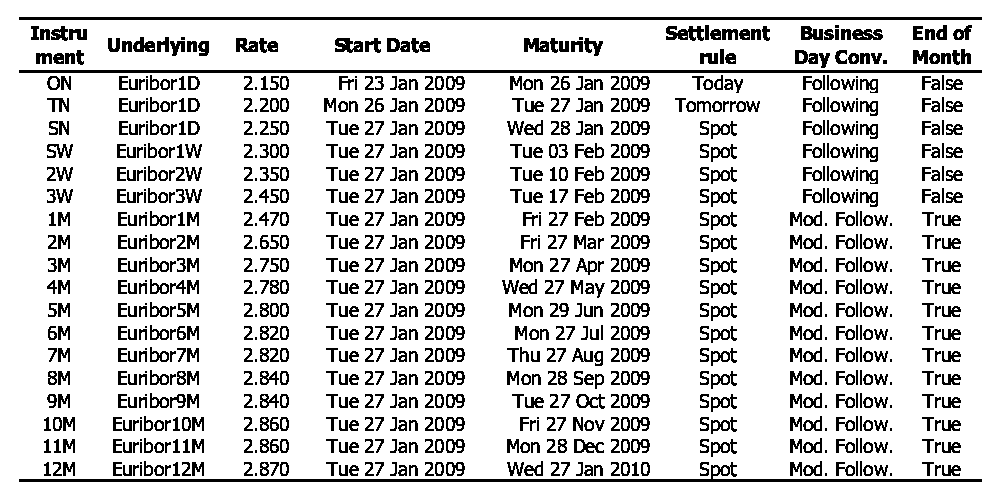
\includegraphics[scale=0.8]{./FigMktDepos}
\caption{EUR Deposit strip. Source: Reuters page KLIEM, 23 Jan. 2009.}
\label{fig:Deposits}
\end{figure}
Interest rate Deposits (Depos) are Over-The-Counter (OTC) zero coupon contracts that start at reference date $t_0$ (today or spot), span the length corresponding to their maturity, and pay the interest accrued over the period with a given rate fixed at $t_0$.
\par
The EUR market quotes standard plain vanilla Deposits strip that start at spot date and span various periods up to 1 year.
Exceptions are the first {\it over-night} (ON) and the second {\it tomorrow-next} (TN) one-day contracts, which start today and tomorrow, respectively, and span one day each, covering (without overlapping) the two business days interval between today and spot dates.
The maturity date of Deposits shorter than one month obeys the {\it following} convention; for longer Deposits the convention is {\it modified following}. For the latters the {\it end-of-month} convention is also respected: if the start date is the last working day in a given month, the end date must be the last working date of the ending month too.
In figure \ref{fig:Deposits} we report the EUR Depo strip quoted in Reuters page KLIEM.
\par
Market Deposits can be selected as bootstrapping instruments for the construction of the short term structure section of the discount curves. Notice that, apart ON, TN and SN, each Depo admits its own underlying rate tenor, corresponding to its maturity. Hence each Depo should be selected, in principle, for the construction of a different curve. We will discuss this point in section \ref{sec:Synt}.
\par
If $R^{Depo}_x\left(t_0,T_i\right)$ is the quoted rate (annual, simply compounded) associated to the i-th Deposit with maturity $T_i$ and underlying rate tenor $x=T_i - t_0$ months, the implied discount factor at time $T_i$ is given by the following relation\footnote{here we keep the subscript $x$ explicit also in order to to be consistent with the following eq. (\ref{eqn:FRA}).}
\begin{equation}
P_x(t_0,T_i) = \frac{1}{1 + R^{Depo}_x\left(t_0,T_i\right)\tau_F\left(t_0,T_i\right)},\quad t_0<T_i,
\label{eqn:Deposit}
\end{equation}
where $\tau_F$ is given by eq. (\ref{eqn:yfFRA}). The expression (\ref{eqn:Deposit}) above can be used to bootstrap the yield curve $\mathcal{C}_x$ at point $T_i$.

\subsubsection{Forward Rate Agreements (FRAs)}
\label{sec:FRA}
[NOTA: aggiungere IMMFRA6M]\\
\begin{figure}[tbp]
\centering
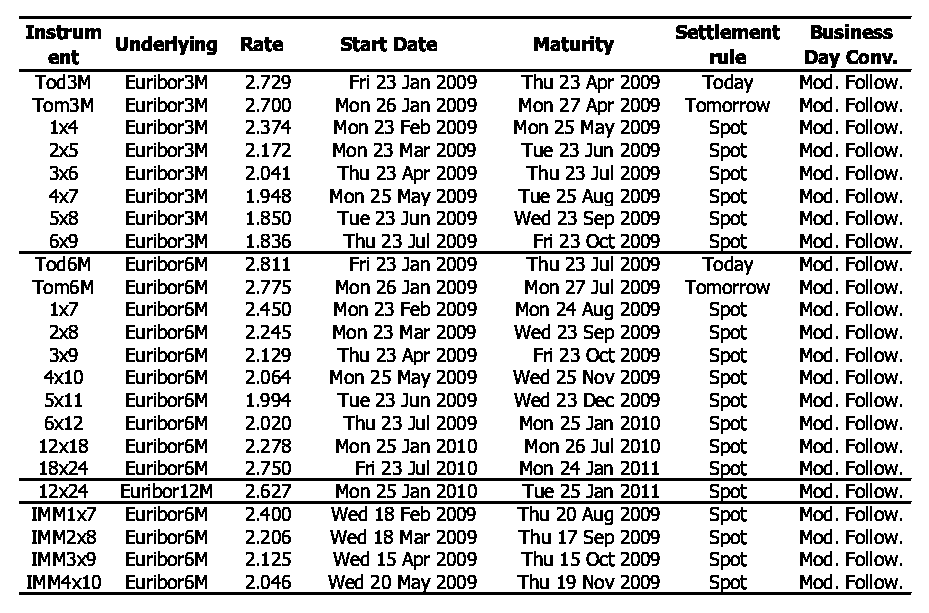
\includegraphics[scale=0.85]{./FigMktFRA}
\caption{EUR FRA strip on Euribor3M, Euribor6M, and Euribor12M. Source: Reuters page ICAPSHORT2, 23 Jan. 2009.}
\label{fig:FRA}
\end{figure}
FRA contacts are forward starting Deposits. For instance the 3x9 FRA is a six months Deposit starting three months forward.
\par
The EUR market quotes standard plain vanilla FRA strips with different forward start dates (i.e. the start date of the forward Depo), calculated with the same convention used for the end date of Deposits. So FRAs do concatenate exactly, e.g. the 6x9 FRA starts when the preceding 3x6 FRA ends. The underlying forward rate fixes two working days before the forward start date (NOTA: VERIFICARE).
In figure \ref{fig:FRA} we report the three FRA strips on 3M, 6M, and 12M Euribor rate quoted in Reuters page ICAPSHORT2.
\par
Market FRAs provide direct empirical evidence that a single curve cannot be used to estimate forward rates with different tenors. We can observe in figure \ref{fig:FRA} that, for instance, the level of the market 1x4 FRA3M (spanning from Feb. 23th to May 25th, $\tau_{F,1x4} = 0.25278$) was $F_{1x4}^{mkt} = 2.374\%$, the level of market 4x7 FRA3M (spanning from May 25th to Aug. 25th, $\tau_{F,4x7} = 0.25556$) was $F_{4x7}^{mkt}=1.948\%$. If one would compound these two rates to obtain the level of the implied 1x7 FRA6M (spanning from Feb. 24th to Aug 24th, $\tau_{F,1x7} = 0.50556$) would obtain
\begin{eqnarray}
F_{1x7}^{implied}
&=& \frac{
    \left(1 + F_{1x4}^{mkt}\tau_{F,1x4}\right) \times
    \left(1 + F_{4x7}^{mkt}\tau_{F,4x7}\right) - 1.0}
    {\tau_{F,1x7}} = 2.178\%,
\label{eqn:FRAarbitrage}
\end{eqnarray}
while the market quote for the $1x7$ FRA6M was $F_{1x7}^{mkt}=2.450\%$, 27 basis point larger. As discussed in section \ref{sec:Pricing}, the difference is the liquidity/default risk premium seen by the market in post credit crunch times.
\par
Market FRAs on $x$-tenor Euribor can be selected, together with the corresponding Depos, as bootstrapping instruments for the construction of the short term structure section of the yield curve $\mathcal{C}_x$.
If $F_x\left(t;T_{i-1},T_i\right)$ is the i-th Euribor forward rate resetting at time $T_{i-1}$ with tenor $x=T_i-T_{i-1}$ months associated to the i-th FRA with maturity $T_i$, the implied discount factor at time $T_i$ is obtained by eq. (\ref{eqn:FwdRate}) as
\begin{equation}
P_x\left(t_0,T_i\right) = \frac{P_x\left(t_0,T_{i-1}\right)}{1+F_{x}\left(t_0;T_{i-1},T_{i}\right)\tau_F\left(T_{i-1},T_{i}\right) },\quad t_0<T_{i-1}<T_i,
\label{eqn:FRA}
\end{equation}
where $\tau_F$ is given by eq. (\ref{eqn:yfFRA}). The expression (\ref{eqn:FRA}) above can be used to bootstrap the yield curve $\mathcal{C}_x$ at point $T_i$ once point $T_{i-1}$ is known.
Notice that FRAs collapse to Depos for shrinking $T_{i-1}-t_0$
\begin{equation}
\lim_{T_{i-1} \to t_0}F_{x}\left(t_0;T_{i-1},T_{i}\right) = R^{Depo}_x\left(t_0,T_i\right),
\end{equation}
and eq. (\ref{eqn:FRA}) reduces to eq. (\ref{eqn:Deposit}).
\par

\subsubsection{Futures}
\label{sec:Futures}
\begin{figure}[tbp]
\centering
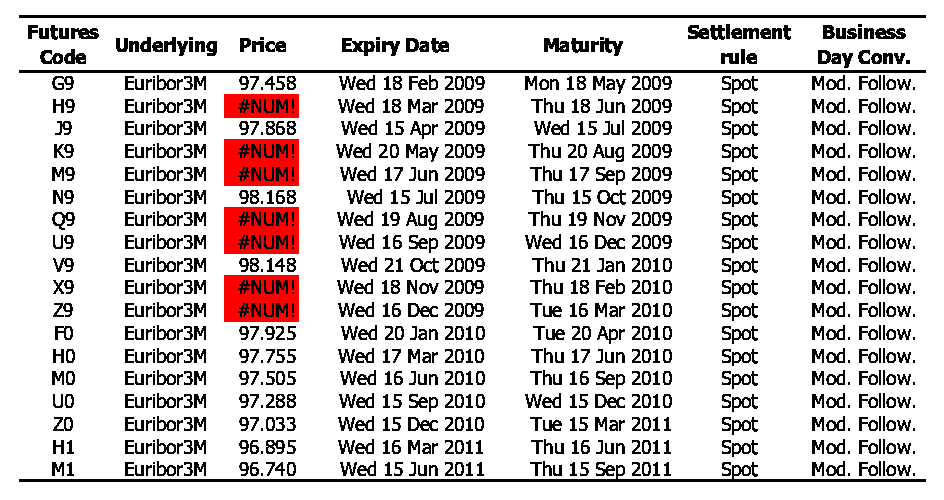
\includegraphics[scale=0.85]{./FigMktFut3M}
\caption{EUR Futures on Euribor 3M. Source: Reuters page 0\#/FEI, 23 Jan. 2009.}
\label{fig:Futures3M}
\end{figure}
Interest Rate Futures are the exchange-traded contracts equivalent to the over-the-counter FRAs. While FRAs have the advantage of being more customizable, Futures are highly standardized contracts. In the EUR market they fix the third Wednesday of the maturity month; the last trading day is the preceding Monday (because of the two days of settlement); the most common contracts (so called IMM\footnote{International Money Market of the Chicago Mercantile Exchange.} Futures) insist on Euribor3M [NOTA: E BASTA ? VERIFICARE] and expire every March, June, September and December (IMM dates). There are also so called serial contracts expiring in the upcoming months not covered by the quarterly Futures. Maturities extend up to 8 years [NOTA: VERIFICARE].
Any profit and loss is regulated through daily marking to market (so called margining process).
\par
Such standard characteristics reduce the credit risk and the transaction costs, thus enhancing a very high liquidity. The first front contract is the most liquid interest rate instrument, with longer expiry contracts having very good liquidity up to the 8th-12th contract. Also the first serial contract is quite liquid, especially when its expiration is before the front contract.
\par
In figure \ref{fig:Futures3M} we report the quoted Futures strip on 3M Euribor rate up to 3 years maturity. As we can see, Futures are quoted in terms of prices instead of rates, the relation being
\begin{equation}
P^{Fut}_x\left(t_0,T_{i-1},T_i\right) = 100 - R^{Fut}_x\left(t_0,T_{i-1},T_i\right),
\label{eqn:FuturePriceRate}
\end{equation}
Because of their marking to market mechanism Futures do not have the same payoff of FRAs: an investor long a Futures contract will have a loss when the Futures price decrease but will finance such loss at lower rate (see \ref{eqn:FuturePriceRate}); viceversa when the Futures price increase the profit will be reinvested at higher rate [NOTA: VERIFICARE]. This means that the volatility of the forward rates and their correlation to the spot rates have to be accounted for, hence a \emph{convexity adjustment} is needed to convert the rate $R^{Fut}_x$ implied in the Futures price to its corresponding forward rate $F_x$,
\begin{equation}
F_x\left(t_0,T_{i-1},T_i\right) = R^{Fut}_x\left(t_0,T_{i-1},T_i\right)-C_x\left(t_0,T_{i-1},T_i\right),
\label{eqn:fwdfromfutureprice}
\end{equation}
The calculation of the convexity adjustment thus requires a model for the evolution of the rates.  While advanced approaches are available in literature (see e.g. refs. \cite{Jac05}, \cite{PitRen06}, \cite{Vaillant}, \cite{BriMer06}), a standard practitioners' recipe is given in ref. \cite{KirNov1997}, based on a simple short rate 1 factor Hull \& White model \cite{HulWhi1990}. This approach has been used in figure \ref{fig:Futures3M} to calculate the adjustments, using fixed Hull-White parameters values as in table \ref{tab:FuturesConAdy}.
\par
Market Futures on $x$-tenor Euribor can be selected as bootstrapping instruments for the construction of short-medium term structure section of the yield curve $\mathcal{C}_x$.
Notice that Futures contracts have expiration dates gradually shrinking to zero and as such they generate rolling pillars that periodically jumps and overlap the fixed Depo and FRA pillars. Hence some \emph{priority} rule must be used in order to decide which instruments must be excluded from the bootstrapping procedure. We will discuss this topic in section \ref{sec:DepoFuturesOverlap}.
\par
Given the i-th Futures market quote $P^{Fut}_x\left(t_0,T_{i-1},T_i\right)$ with maturity $T_i$, the implied discount factor at time $T_i$ is obtained by eqs. (\ref{eqn:FRA}), (\ref{eqn:FuturePriceRate}) and (\ref{eqn:fwdfromfutureprice}) as
\begin{equation}
P_x\left(t_0,T_i\right)
=   \frac{P_x\left(t_0,T_{i-1}\right)}
         {1+\left[R^{Fut}_x\left(t_0,T_{i-1},T_i\right) -
          C_x\left(t_0,T_{i-1},T_i\right)\right]
          \tau_F\left(T_{i-1},T_{i}\right)},
\label{eqn:FuturesBootstrap}
\end{equation}
where $\tau_F$ is given by eq. (\ref{eqn:yfFRA}). The expression above can be used to bootstrap the yield curve $\mathcal{C}_x$ at point $T_i$ once point $T_{i-1}$ is known.

\begin{table}[tbp]
\begin{tabular}{lc}
\midrule
HW parameter   & Value \\
\midrule
Mean reversion & 0.03  \\
Volatility & 0.827\%   \\
\midrule
\end{tabular}
\caption{Hull-White parameters values for Futures3M convexity adjustment at 23 Jan. 2009. [NOTA: specificare come sono stati calibrati]}
\label{tab:FuturesConAdy}
\end{table}

\subsubsection{Swaps}
\label{sec:Swap}
Interest rate Swaps are Over-The-Counter (OTC) contracts in which two counterparties agree to exchange fixed against floating rate cash flows. These payment streams are called fixed and floating leg of the Swap, respectively.
\par
The EUR market quotes standard plain vanilla Swaps starting at spot date with annual fixed leg and floating leg indexed to x-months Euribor rate with x-months frequency. In this case the Swap can be regarded as a portfolio of FRA contracts (the first one is actually a Deposit). The day count convention for the quoted (fair) swap rates is \emph{30/360 (bond basis)} \cite{ISDA}.
In figures \ref{fig:Swaps6M}, \ref{fig:SwapsIMM} and \ref{fig:Swaps1M} we report the quoted Swaps strips on 6M, 3M and 1M Euribor rates, respectively.
\par
Market Swaps on $x$-tenor Euribor can be selected as bootstrapping instruments for the construction of the medium-long term structure section of the yield curve $\mathcal{C}_x$.
Given the swap rate $S_x\left(t_0,T_i\right)$ quoted for maturity $T_i$, from equation (\ref{eqn:SwapRateFwd}) we obtain, setting $T_0=S_0=t=t_0$ and $T_n=S_m=T_i$,
\begin{eqnarray}
S_x\left(t_0,T_i\right)
&=& \frac{1 - P_x\left(t_0,T_i\right)}
         {A_x\left(t_0,T_i\right)} \notag\\
&=& \frac{1 - P_x\left(t_0,T_i\right)}
         {A_x\left(t_0,T_{i-1}\right)+P_x\left(t_0,T_i\right)\tau_S\left(T_{i-1},T_i\right)}.
\label{eqn:SwapRateMkt}
\end{eqnarray}
The expression above can be inverted to find the implied discount factor at time $T_i$ as
\begin{equation}
P_x\left(t_0,T_i\right)
=   \frac{1-S_x\left(t_0,T_i\right)A_x\left(t_0,T_{i-1}\right)}
         {1+S_x\left(t_0,T_i\right)\tau_S\left(T_{i-1},T_i\right)},
\label{eqn:SwapBootstrap}
\end{equation}
where $\tau_S$ is given by
\begin{equation}
\tau_S\left(T_1,T_2\right) := \tau\left[T_1,T_2;30/360 (bond basis)\right].
\end{equation}
Expression (\ref{eqn:SwapBootstrap}) can be used to bootstrap the yield curve $\mathcal{C}_x$ at point $T_i$ once the points $\mathbf{T=}\left\{T_1,...,T_{i-1}\right\}$ are known.

TBD: liquid Swaps and interpolated ones

\begin{figure}[tbp]
\centering
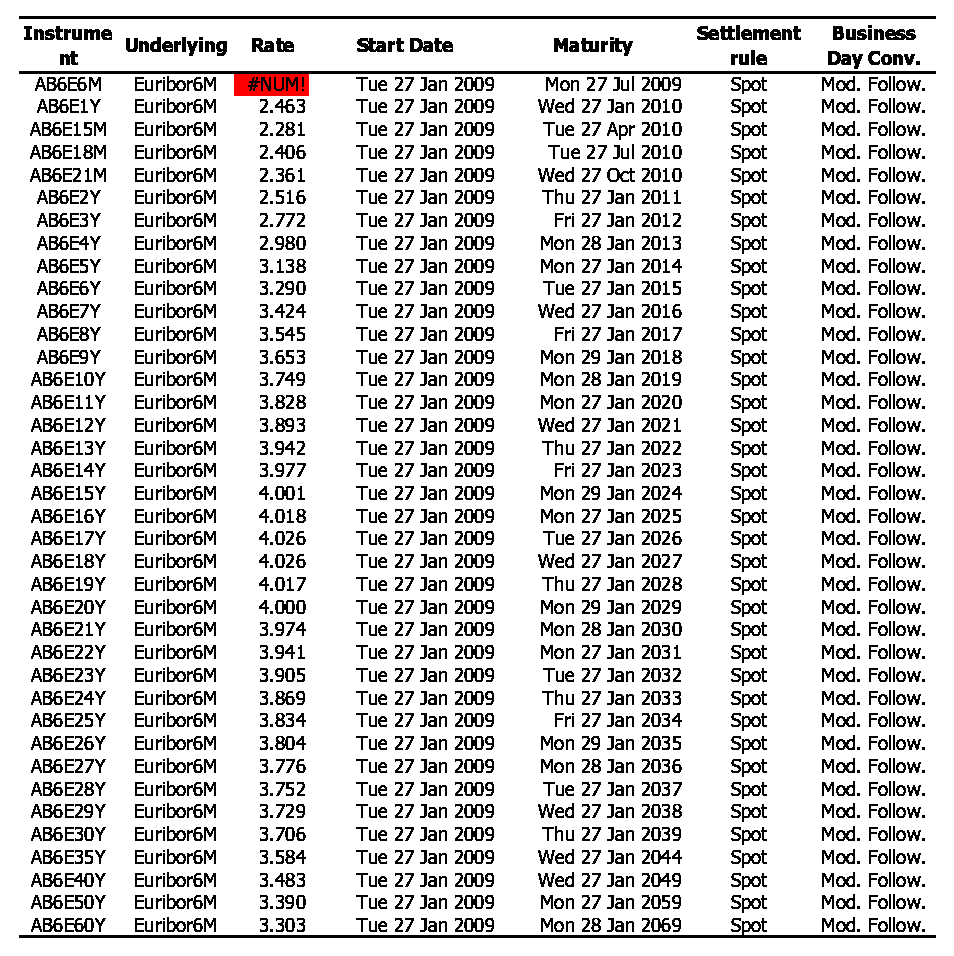
\includegraphics[scale=0.85]{./FigMktSwaps6M}
\caption{EUR Swaps on Euribor6M. Source: Reuters page ICAPEURO, 23 Jan. 2009.}
\label{fig:Swaps6M}
\end{figure}

\begin{figure}[tbp]
\centering
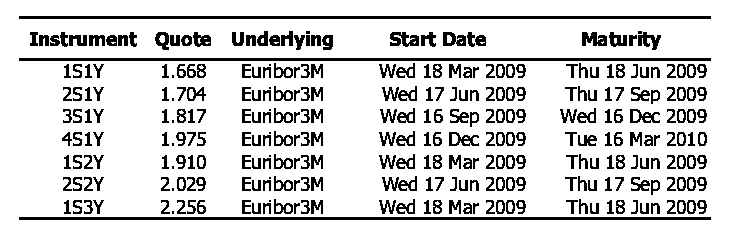
\includegraphics[scale=0.85]{./FigMktSwapsIMM}
\caption{EUR IMM Swaps on Euribor3M. Source: Reuters page ICAPSHORT2, 23 Jan. 2009.}
\label{fig:SwapsIMM}
\end{figure}

\begin{figure}[tbp]
\centering
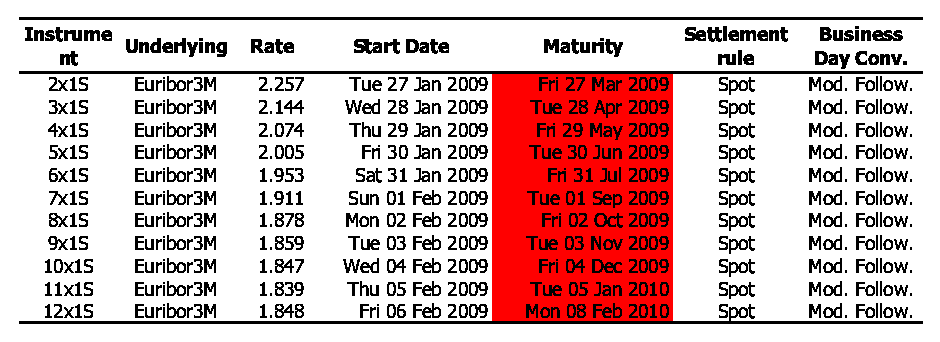
\includegraphics[scale=0.85]{./FigMktSwaps1M}
\caption{EUR Swaps on Euribor1M. Source: Reuters page ICAPSHORT2, 23 Jan. 2009.}
\label{fig:Swaps1M}
\end{figure}

\subsubsection{Basis Swaps}
\begin{figure}[tbp]
\centering
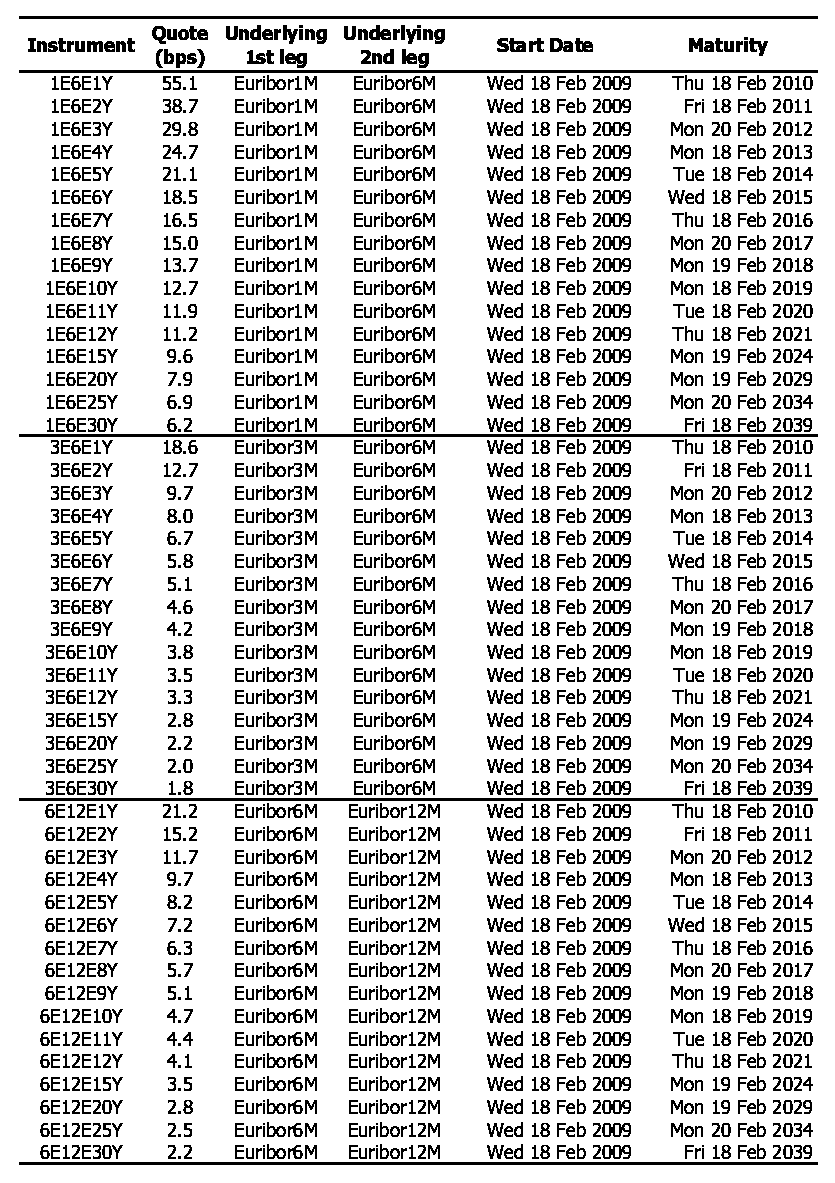
\includegraphics[scale=0.85]{./FigMktBasis}
\caption{EUR Basis Swaps. Source: Reuters page ICAPEUROBASIS, 23 Jan. 2009.}
\label{fig:BasisSwaps}
\end{figure}
\begin{figure}[tbp]
\centering
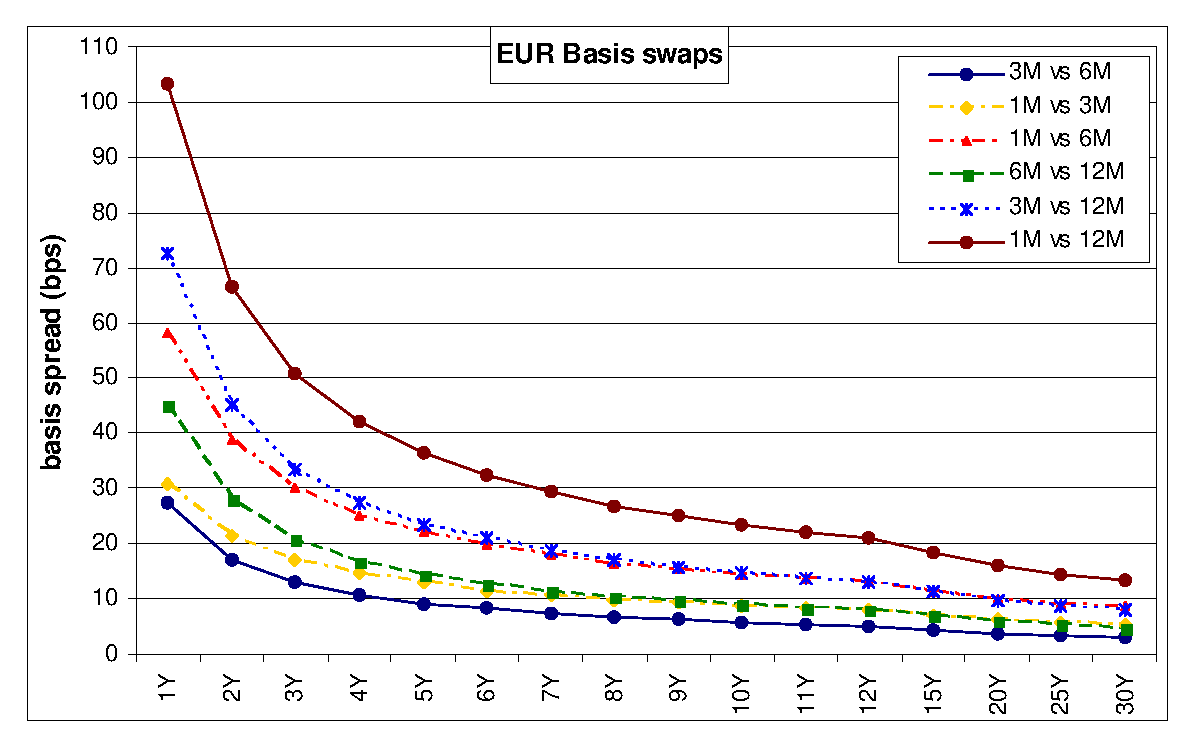
\includegraphics[scale=0.65]{./FigMktBasisSwapsGraph}
\caption{EUR Basis Swaps from figure \ref{fig:BasisSwaps}. The other basis have been deduced using eq. (\ref{eqn:BasisSwap}).}
\label{fig:BasisSwapsGraph}
\end{figure}
Interest rate (single currency) Basis Swaps are floating vs floating swaps admitting underlying rates with different tenors.
\par
The EUR market quotes standard plain vanilla Basis Swaps as portfolios of two swaps with the same fixed legs and floating legs paying Euribor xM and yM, e.g. 3M vs 6M, 1M vs 6M, 6M vs 12M, etc.
In figure \ref{fig:BasisSwaps} we report three quoted Basis Swaps strips.
The quotation convention is to provide the difference (in basis points) between the fixed rate of the lower frequency swap and the fixed rate of the higher frequency swap. At the moment such difference is positive and decreasing with maturity, reflecting the preference of market players for receiving payments with higher frequency (3M instead of 6M, for instance) and short maturities.
\par
Basis swaps are a fundamental element for multi curve bootstrapping, because, starting from the quoted Swaps on Euribor 6M (figure \ref{fig:Swaps6M}), they allow to imply levels for non-quoted Swaps on Euribor 1M, 3M, and 12M, to be selected as bootstrapping instruments for the corresponding yield curves construction.
If $\Delta_{x,6M}\left(t_0,T_i\right)$ is the quoted basis between Euribor xM and Euribor 6M for maturity $T_i$ we have
\begin{equation}
S_x\left(t_0,T_i\right) = \Delta_{x,6M}\left(t_0,T_i\right) + S_{6M}\left(t_0,T_i\right),
\label{eqn:BasisSwap}
\end{equation}
with the obvious caveat that
$\Delta_{6M,x}\left(t_0,T_i\right) = - \Delta_{x,6M}\left(t_0,T_i\right)$. Obviously, non quoted basis can be deduced as
\begin{eqnarray}
\Delta_{x,y}\left(t_0,T_i\right) &=& S_x\left(t_0,T_i\right)-S_y\left(t_0,T_i\right),\notag\\
\Delta_{y,z}\left(t_0,T_i\right) &=& S_y\left(t_0,T_i\right)-S_z\left(t_0,T_i\right),\notag\\
\Delta_{x,z}\left(t_0,T_i\right) &=& \Delta_{x,y}\left(t_0,T_i\right)+\Delta_{y,z}\left(t_0,T_i\right).
\label{eqn:BasisSwap2}
\end{eqnarray}
We have reported all the possible combinations in figure \ref{fig:BasisSwapsGraph}.

\subsection{The Deposits-Futures Overlap (TBD)}
\label{sec:DepoFuturesOverlap}\par
[NOTA: descrivere i vari modi per gestire il raccordo fra Depositi e Futures ?]

\subsection{\label{sec:Interp}The Role of Interpolation (TBD)}
\par
The interpolation we choose for the given parametrization determines how reasonable the yield curve will be. For instance, linear interpolation of the discount factors is an obvious but extremely poor choice. Linear interpolation of zero rates or log-discounts are popular choices leading to stable and fast bootstrapping procedures. Unfortunately they produce discontinuous forward rates, with a sagsaw or piecewise-constant shape.

flat extrapolation out to infinity.

well-documented problems with spurious inflection points, excessive convexity, and lack of locality in the effects of input price perturbations. Andersen \cite{And07} addresses these issues through the use of shape-preserving splines from the class of generalized tension splines.

Swap selection

liquid Swaps and interpolated ones

citare Hyman \cite{Hym1983}, \cite{HagWes06}, \cite{HagWes08}).

TBD: mostrare casi di cattiva interpolazione, ad es. linear on zero rates


\subsection{\label{sec:TOY}The Turn-of-Year Effect (TBD)}
\par
TBD

\subsection{\label{sec:Synt}Synthetic Instruments (TBD)}
\par
TBD
problema dello scodamento. e sua soluzione tramite synthetic Depos


\section{Implementation and Numerical Results (TBD)}
\label{sec:ImplementResults}

\subsection{Implementation (TBD)}
\label{sec:Implementation}
The results discussed above have been obtained by the authors using the QuantLib framework. The object oriented C++ QuantLib library \cite{QuantLib} offers tools for advanced modeling and practical implementation, with features such as market conventions, yield curve models, solvers, PDEs, (Quasi)\ Monte Carlo, exotic options, VAR, etc. The QuantLibAddin \cite{QuantLibAddin} and QuantLibXL \cite{QuantLibXL} projects use the ObjectHandler in-memory repository \cite{ObjectHandler} to export the QuantLib objects (classes) and analytic (methods) to a variety of end-user platforms including Excel and Calc. The full implementation of the work described before, comprehensive of C++ code and Excel workbooks, is open source. In particular...
[\emph{TBD: ampliare questo punto descrivendo meglio che cosa \`{e} effettivamente implementato e disponibile ?\ }]. Anyone interested in the topic is invited to post to the QuantLib community any comment or suggestion to improve the job.

\subsection{Numerical Results (TBD)}
\par
Inserire 4 figure con il bootstrapping delle 4 curve (strumenti, scadenze, tassi)\\
Inserire tests di repricing degli strumenti sulle 4 curve ??
\begin{figure}[tbp]
\centering
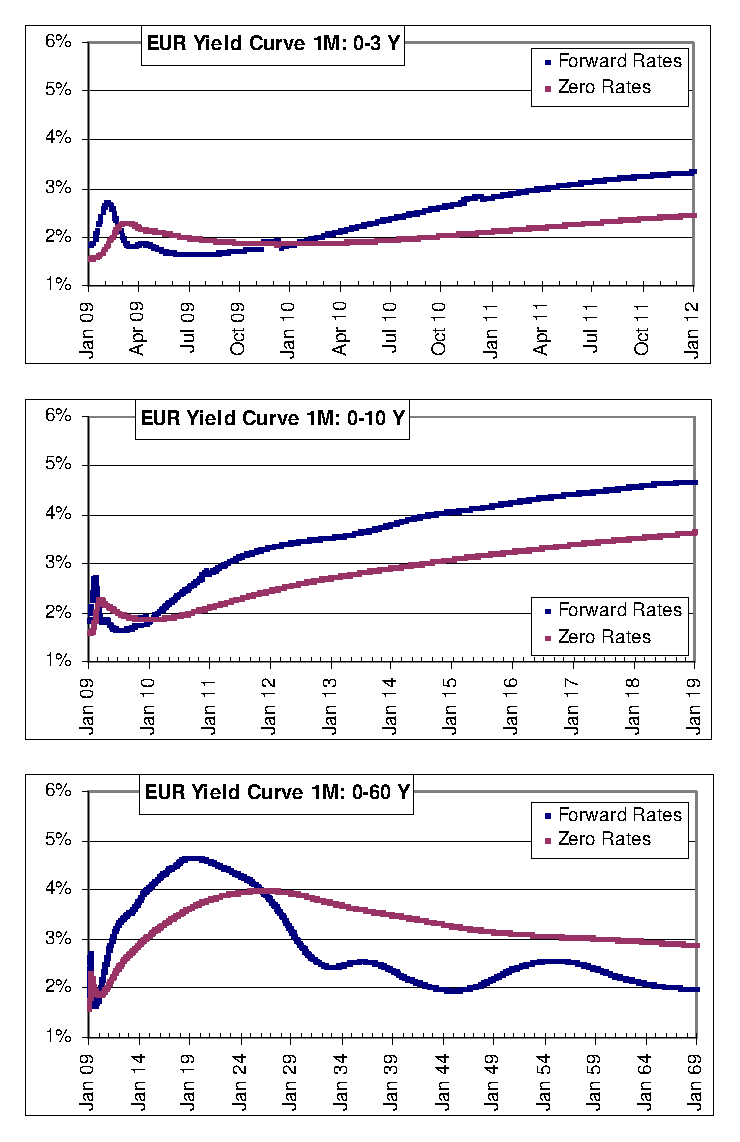
\includegraphics[scale=0.9]{./FigYC1M}
\caption{Yield curve on Euribor1M. Brown line: zero curve, plotted with zero rates $Z_{f}^{I_{1M}}\left(t_{0},t_{0}+t,\text{\textit{act/365}}\right)$, $t$ daily sampled and spot date $t_{0}=$ Jan. 27th, 2009. Blu line: forward curve $\mathcal{C}_{I_{1M}}^f$, plotted with 1M-tenor forward rates $F\left( t_{0};t,t+1M,\text{\textit{act/360}}\right) $. Upper panel: short term structure up to 3 years; middle panel: medium term structure up to 10 years; lower panel: long term structure up to 60 years.}
\label{FigYC1M}
\end{figure}

\begin{figure}[tbp]
\centering
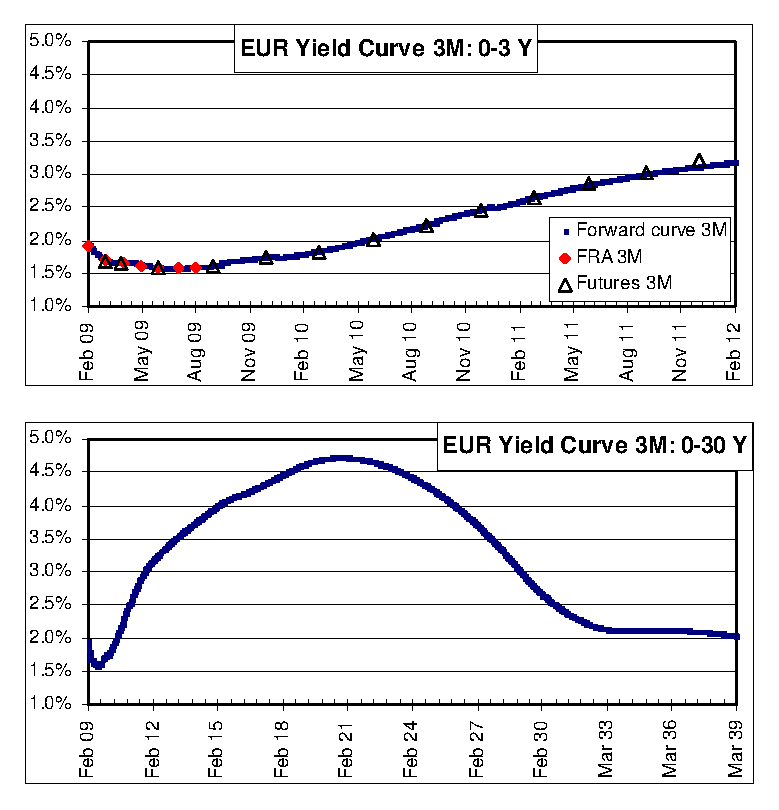
\includegraphics[scale=0.9]{./FigYC3M}
\caption{Yield curve on Euribor3M. Plots as in fig. \protect\ref{FigYC1M}. Cyan diamonds: quoted 3M FRAs. Green triangles: quoted 3M\ Futures.}
\label{FigYC3M}
\end{figure}

\begin{figure}[tbp]
\centering
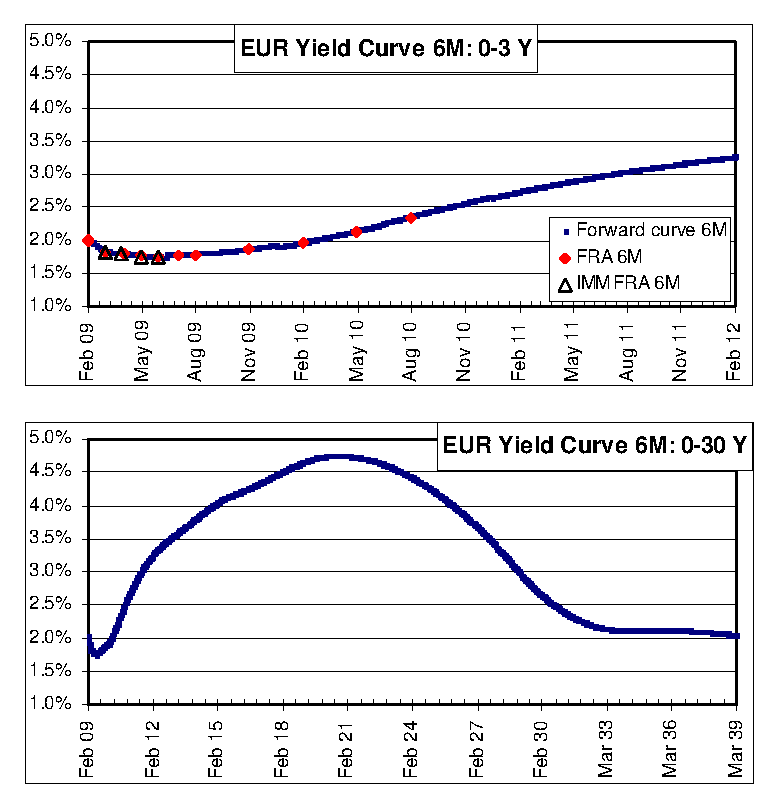
\includegraphics[scale=0.9]{./FigYC6M}
\caption{Yield curve on Euribor6M. Plots as in fig. \protect\ref{FigYC1M}. Cyan diamonds: quoted 6M FRAs. Green triangles: quoted 6M\ Futures.}
\label{FigYC6M}
\end{figure}

\begin{figure}[tbp]
\centering
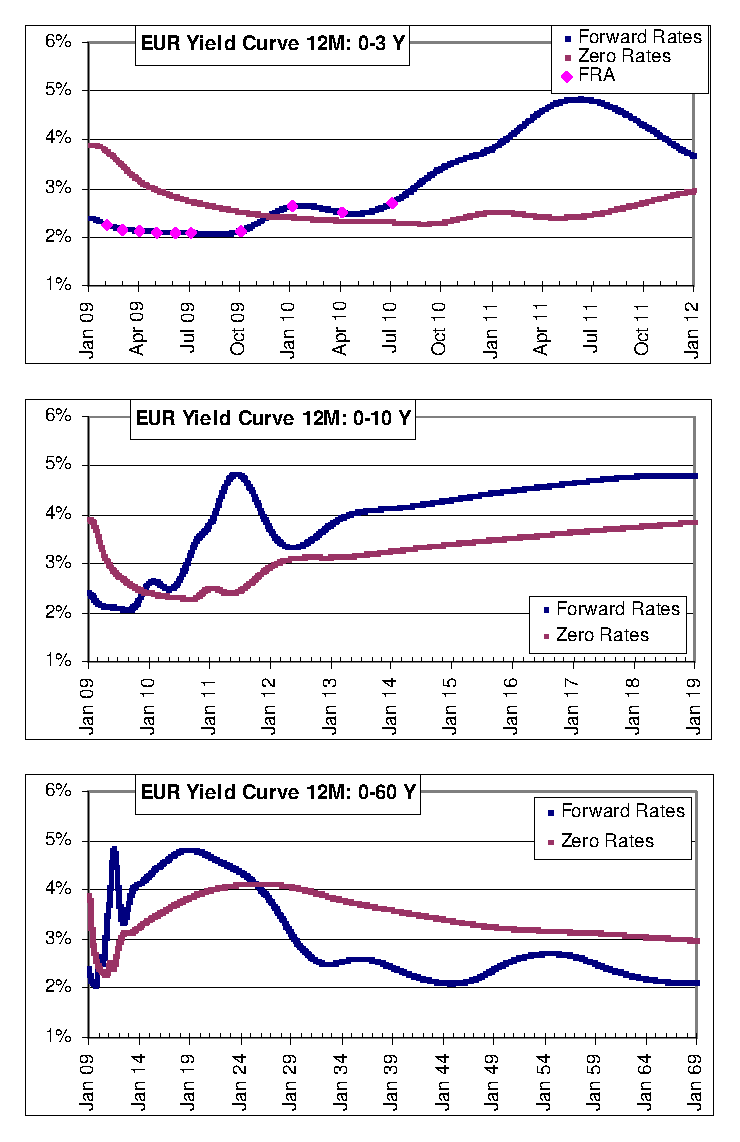
\includegraphics[scale=0.9]{./FigYC12M}
\caption{Yield curve on Euribor12M. Plots as in fig. \protect\ref{FigYC1M}. Cyan diamonds: quoted 12M FRAs.}
\label{FigYC12M}
\end{figure}

\section{Pricing Interest Rate Derivatives Using Separated Yield Curves for Discounting and Forwarding (TBD)}
\label{sec:Pricing2curves}
In this section we revisit the general problem of pricing interest rate derivatives using two different yield curves for discounting and forwarding.
\\
mettere solo cenni a quanto c'e' nell'altro paper.


\subsection{Quanto Adjustment (TBD)}
\label{sec:QuantoAdj}
TBD


\section{Conclusions (TBD)}
\label{sec:Conclusions}
TBD


\bibliographystyle{unsrt}
\bibliography{FinanceBibliography}

\end{document}
